\begin{figure*}[htbp]
    \centering
    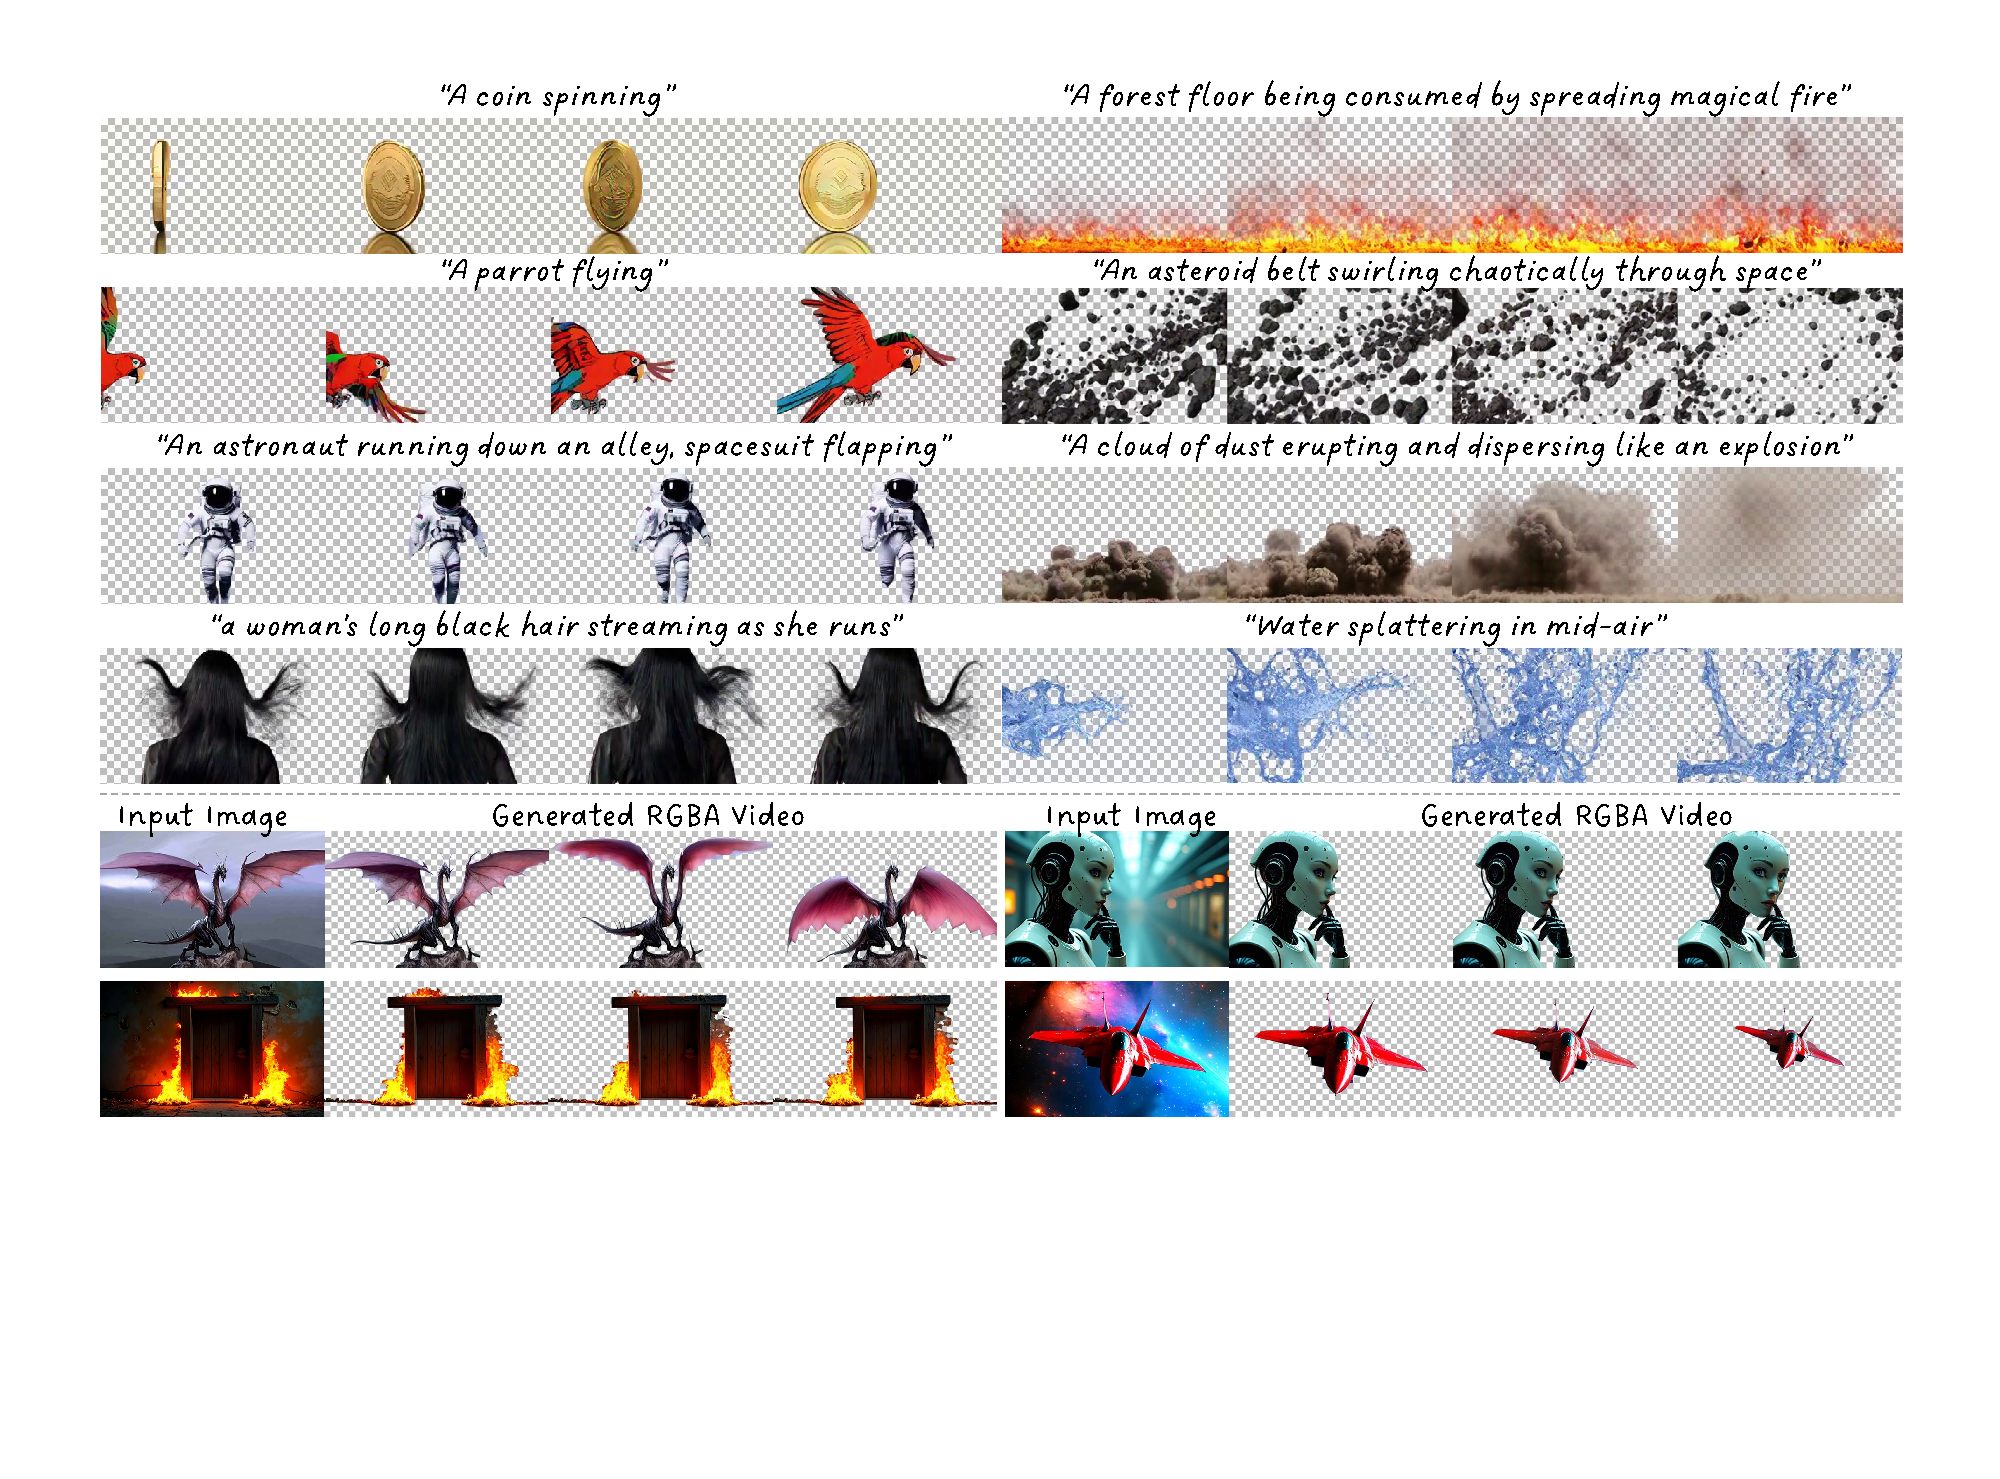
\includegraphics[width=1.0\linewidth]{figs/exp-applications.pdf}
    \vspace{-0.2in}
    \caption{\textbf{Applications.} \textbf{Top}: Text-to-Video with Transparency. \textbf{Bottom}: Image-to-Video generation with transparency.
.}
    \label{fig-applications}
    \vspace{-0.1in}
\end{figure*}


\section{Experiment}
\label{sec:exp}

%-------------------------------------------------------------------------
%\subsection{Implementation Details}

\noindent\textbf{Training Dataset.}~We utilize the public VideoMatte240K dataset~\cite{lin2021real}, a comprehensive collection of 484 high-resolution green screen videos consists of 240,709 unique frames of alpha mattes and foregrounds. These frames provide a diverse range of human subjects, clothing styles, and poses. We apply fundamental preprocessing steps for them, including color decontamination and background blurring. Prompts are extracted using ShareGPT4V~\cite{chen2023sharegpt4v}. 

\vspace{0.5em}
\noindent\textbf{Model.}~Our RGBA video diffusion models are developed by fine-tuning pre-trained diffusion models. Specifically, we employ two models based on the diffusion transformer architecture: the open-source model CogVideoX~\cite{yang2024cogvideox} and a modified variant of CogVideoX denoted as \(J\). 
CogVideoX generates RGB videos at a resolution of 480x720 with 49 frames at 8 FPS, using 50 sampling steps. In contrast, the modified version produces videos at a resolution of 176x320 with 64 frames at 24 FPS, while also using 50 sampling steps. Additionally, we integrate our method with CogVideoX-I2V (Image-to-Video) to support image-to-video generation with transparency.
We set the LoRA rank to 128. For domain embedding, we initialize it with an original shape of \(1\times D\) and zero values, then expand it to \(L\times D\) through repetition during training. 
We train these parameters over 5,000 iterations with a batch size of 8 in total, utilizing 8 NVIDIA A100 GPUs.



\begin{figure*}[htbp]
    \centering
    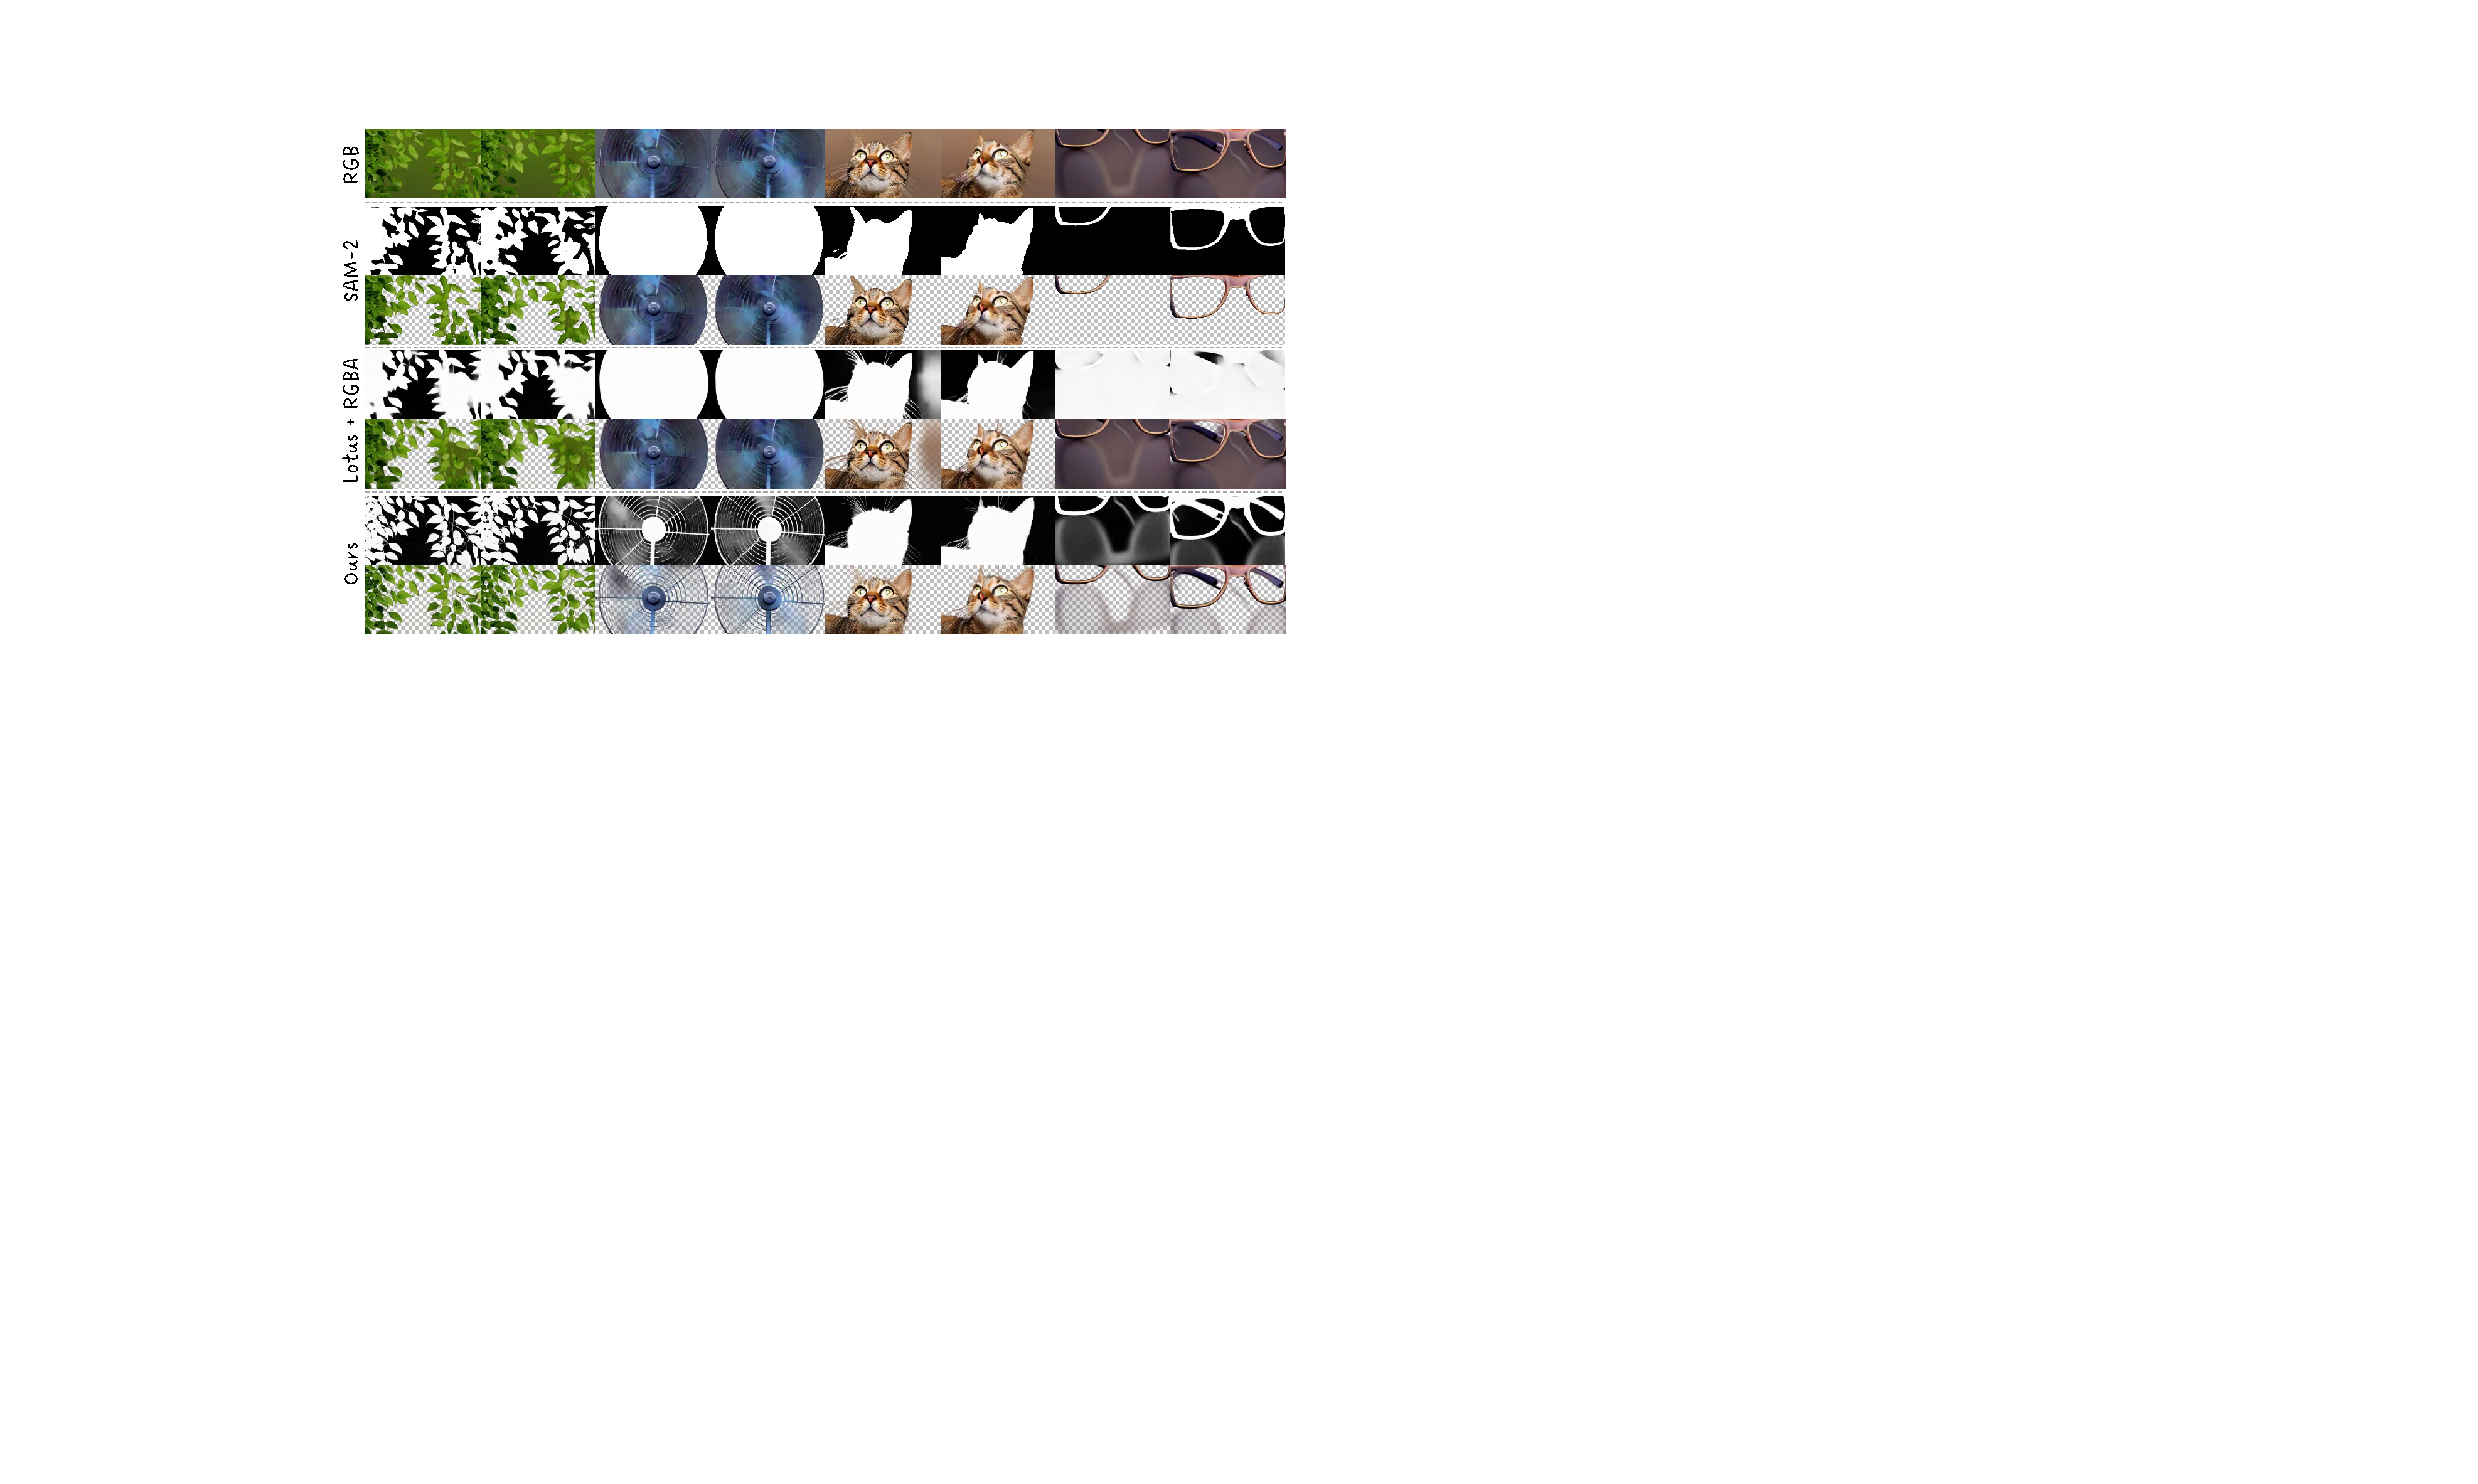
\includegraphics[width=1.0\linewidth]{figs/exp-comparison.pdf}
    \vspace{-0.2in}
    \caption{\textbf{Comparison with Generation-then-Prediction Pipelines.} Our method demonstrates superior alignment.
}
    \label{fig-comparison}
\end{figure*}

\begin{figure*}[htbp]
    \centering
    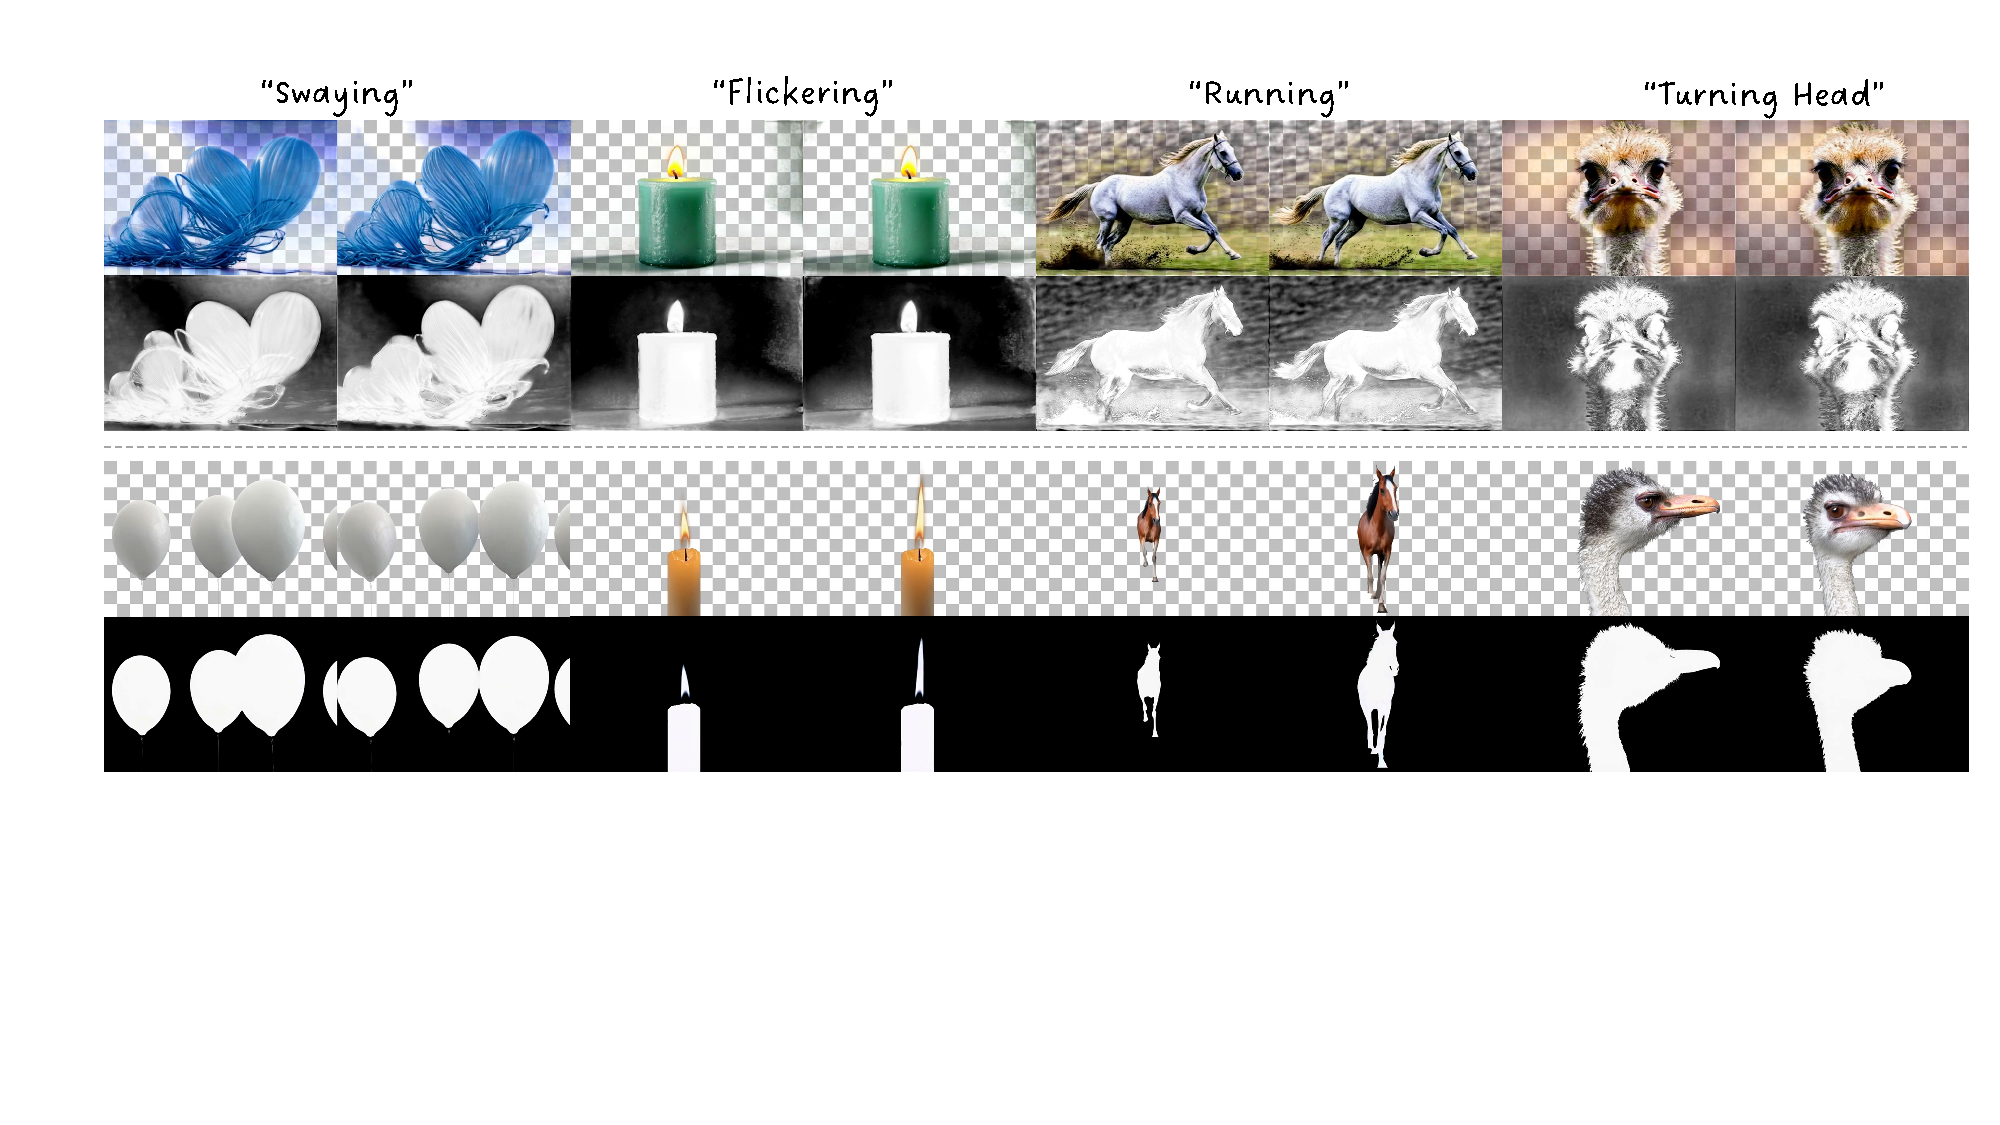
\includegraphics[width=1.0\linewidth]{figs/exp-comparison-generation.pdf}
    \caption{\textbf{Comparison with Joint Generation Pipelines.} \textbf{Top}: LayerDiffusion + AnimateDiff; \textbf{Bottom}: Ours. Our method achieves better alignment and generates corresponding motion described by prompts.}
    \label{fig-comparison-generation}
    \vspace{-0.1in}
\end{figure*}

% %-------------------------------------------------------------------------
\subsection{Applications}
We mainly demonstrate two applications shown in Fig.~\ref{fig-applications}: 

\vspace{0.5em}
\noindent\textbf{Text-to-Video with Transparency.}~Our method is capable of generating moving objects with various types of motion, such as spinning, running, and flying, while also handling transparent properties of bottles and glasses. Additionally, it can produce complex visual effects, including fire, explosions, cracking, and lightning, as well as creative examples.

\vspace{0.5em}
\noindent\textbf{Image-to-Video with Transparency.}~Our method can also be integrated with an I2V video generation model-CogVideoX-I2V. Users can provide a single image along with an alpha channel (optional), and then we generate subsequent frames with dynamic effects and automatically propagate or generate alpha channels for these frames.



% %-------------------------------------------------------------------------
\subsection{Comparisons}

% \noindent\textbf{Generation-then-Prediction Pipeline.}~We compare our method with a generation-then-prediction pipeline. We first run our approach, denoted as \( J \), to generate both RGB and alpha channels. Then, we apply various prediction models to infer the alpha channel based on the generated RGB frames. For our main baselines, we use Lotus~\cite{he2024lotus} and SAM-2~\cite{ravi2024sam2}, which either leverage pretrained RGB models or are trained on large datasets. Since Lotus was originally designed for single-image depth estimation, we adapt its framework for application within our video generation model (\( J \)). For comparisons with video matting methods~\cite{lin2021real,qin2023bimatting,yao2024matte}, which are trained exclusively on human portraits and lack generalizability to other objects, please refer to the supplementary materials.
\noindent\textbf{Generation-then-Prediction Pipeline.}~As shown in Fig.~\ref{fig-intro}, video matting methods~\cite{lin2021real,qin2023bimatting,yao2024matte} struggle with matting non-human objects (see supplementary materials for additional results). Therefore, we selected Lotus~\cite{he2024lotus} and SAM-2~\cite{ravi2024sam2} as baselines due to their stronger generalization: Lotus uses pretrained generative models, and SAM-2 is trained on large datasets. Since Lotus was originally designed for single-image depth estimation, we extended it for RGBA videos, denoted as Lotus + RGBA in our comparisons. Qualitative results are shown in Fig.~\ref{fig-comparison}. Since ground-truth alpha channels are not available for generated videos, we focus on qualitative comparison. 


\vspace{0.5em}
\noindent\textbf{Joint Generation Pipeline.}~Since there are currently no existing RGBA video generation models, we integrate AnimateDiff~\cite{guo2023animatediff} with LayerDiffusion~\cite{zhang2024transparent} to generate RGBA videos. We use the open-source video generation model CogVideoX~\cite{yang2024cogvideox} as the base model for fair comparison. 
The qualitative results are illustrated in Fig.~\ref{fig-comparison-generation}.


\vspace{0.5em}
\noindent\textbf{User Study.}~
We also conduct a user study with Amazon Mechanical Turk to compare two joint generation methods, as shown in Table.~\ref{tab:user_study}. Participants are asked to evaluate two key aspects: 1) whether the RGB and alpha align correctly; and 2) whether the motion in the generated video matches the corresponding text description. A total of 30 videos are generated from distinct text prompts, and 87 users participated in the evaluation. The study shows that our method is obviously favored more by users with higher votes.

\begin{table}
    \centering
    \caption{\textbf{User Study.}}
    \vspace{-0.1in}
    \resizebox{1.0 \columnwidth}{!}{%
    \begin{tabular}{ccc} \toprule
         &RGBA Alignment  &Motion Quality \\ \toprule AnimateDiff~\cite{guo2023animatediff}+LayerDiff~\cite{zhang2024transparent}& 6.7\% &21.7\% \\ 
         Ours + CogVideoX~\cite{yang2024cogvideox}& \textbf{93.3\%} &\textbf{78.3\%} \\ \bottomrule
    \end{tabular}
    }
    \vspace{-0.1in}
    \label{tab:user_study}
\end{table}



% %-------------------------------------------------------------------------
\subsection{Ablation Study}
\begin{figure}[htbp]
    \centering
    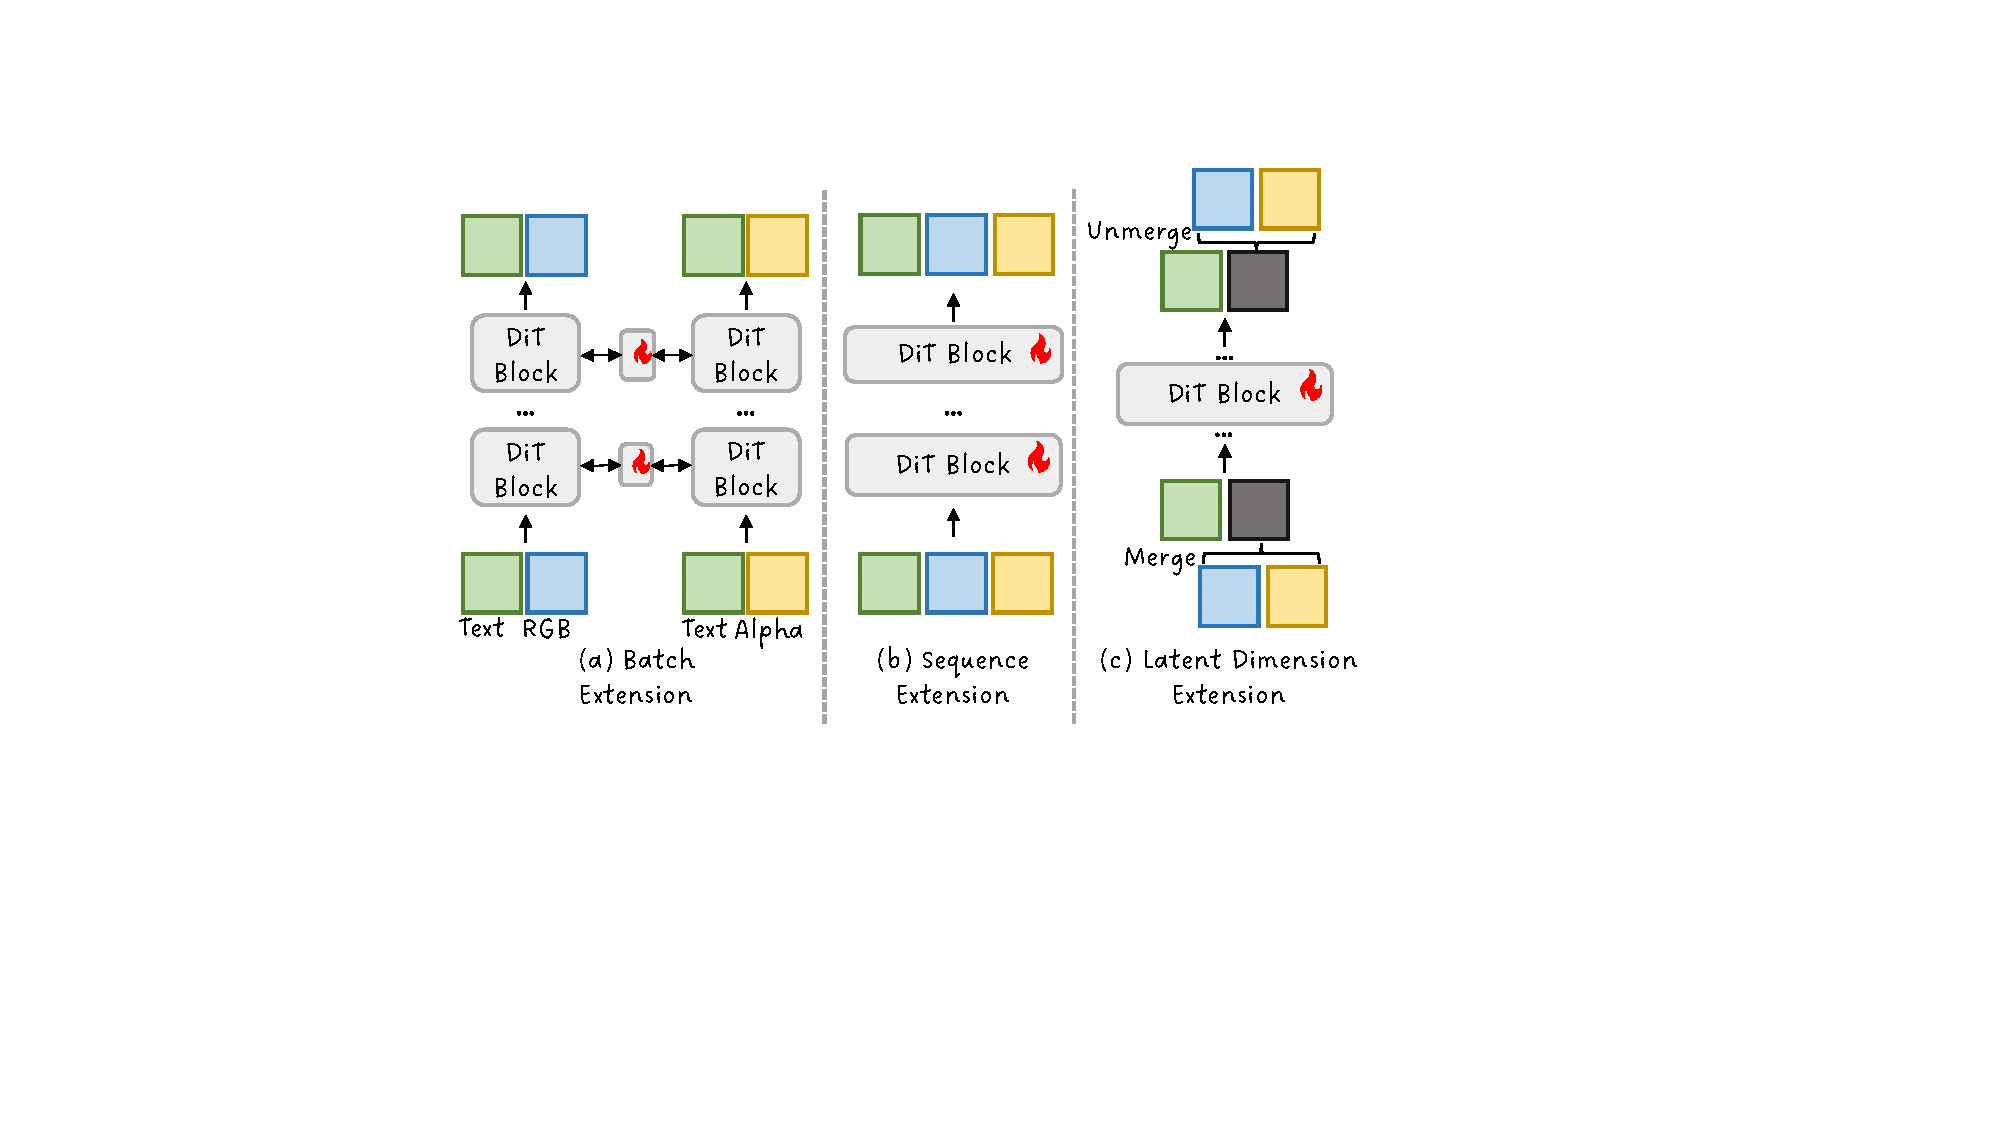
\includegraphics[width=1.0\linewidth]{figs/discussions.pdf}
    \caption{\textbf{Alternative Designs for Joint Generation with DiT}. Sequence extension (b) represents our method.}
    \label{fig-arch}
\end{figure}
As shown in Fig.~\ref{fig-ablation}, we conduct the ablation study across two dimensions: attention rectification and network design.
\begin{figure}[h]
    \centering
    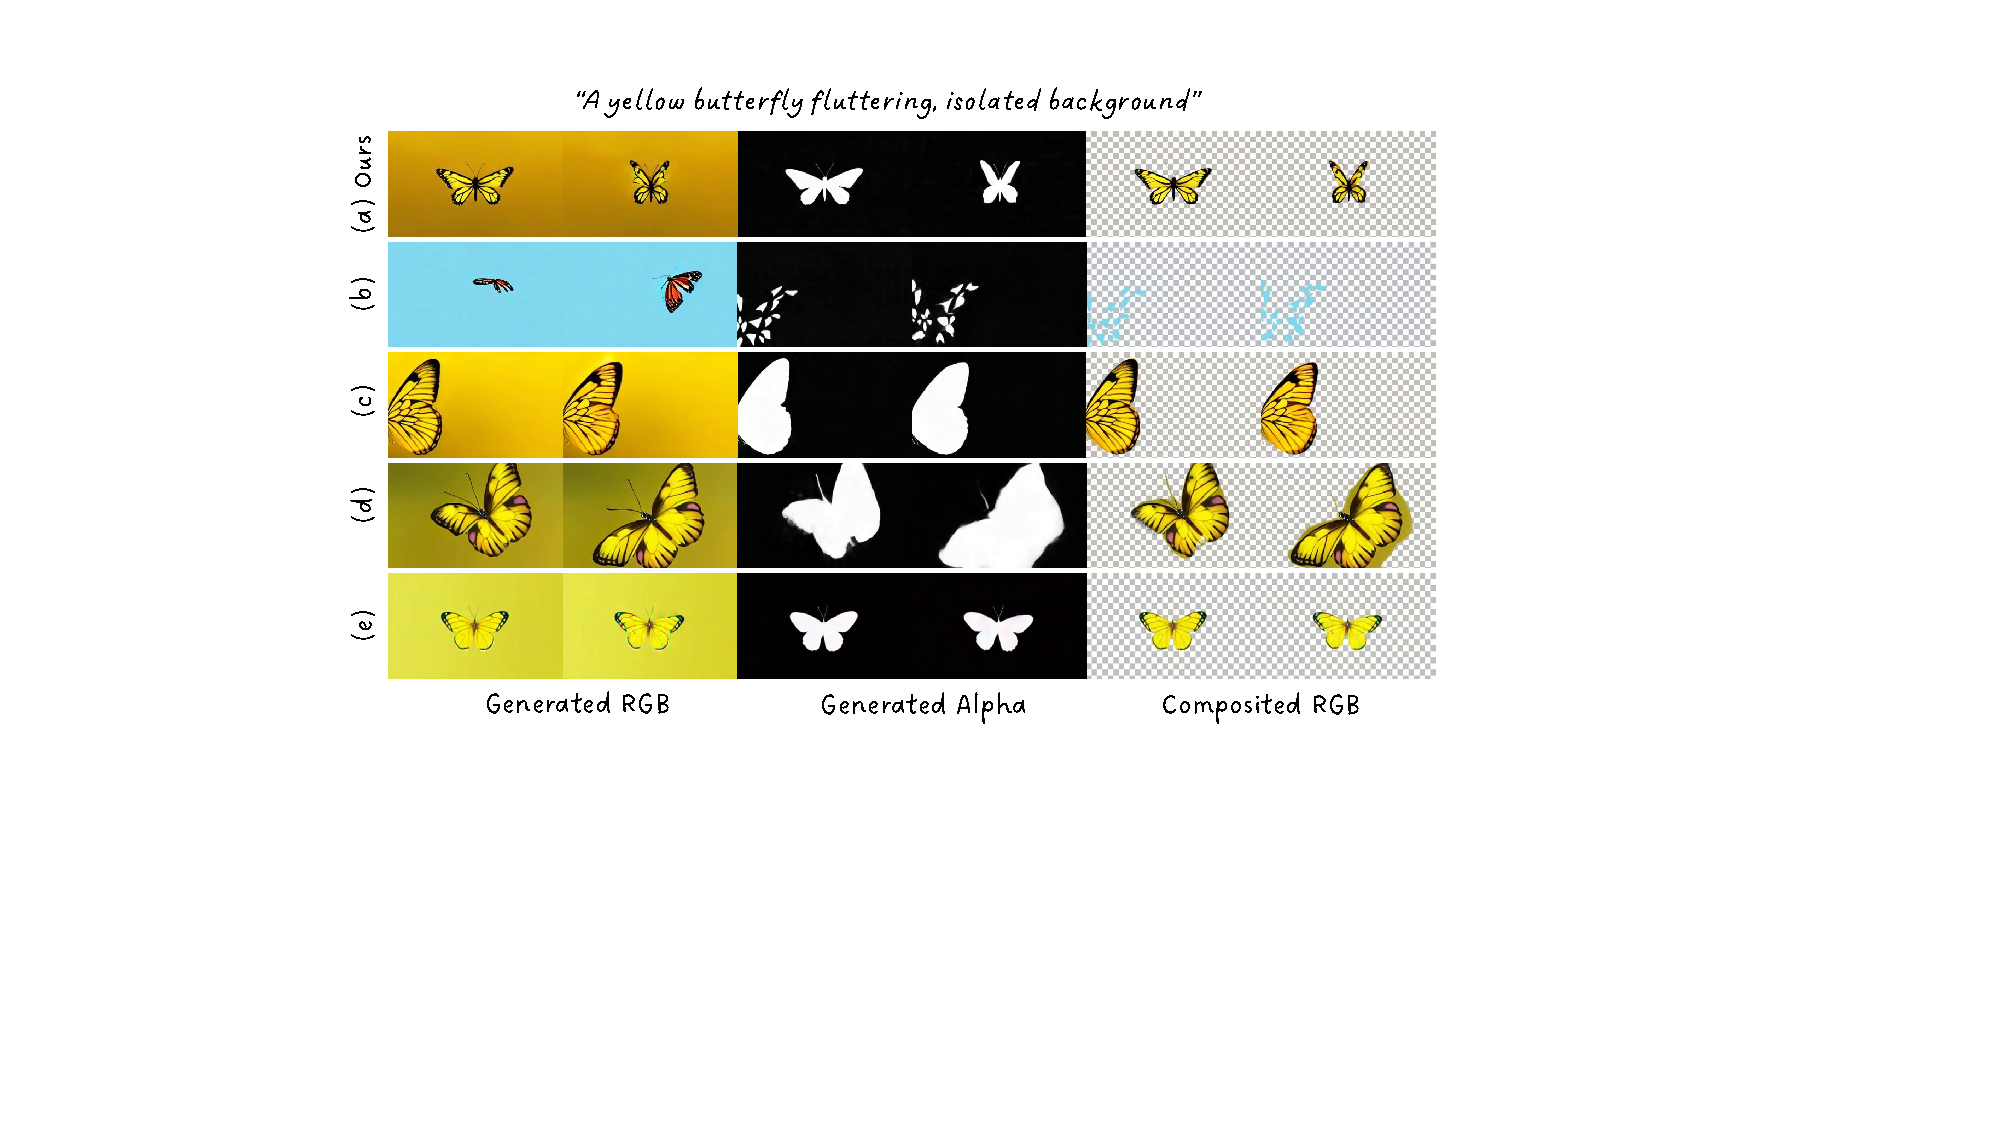
\includegraphics[width=1.0\linewidth]{figs/exp-ablation.pdf}
    \caption{\textbf{Ablation Study.} (a) Ours; (b) Ours without RGB-attend-to-Alpha; (c) Ours with Text-attend-to-alpha; (d) Batch Extension Strategy; (e) Latent Dimension Extension Strategy. Our method maintains high-quality motion generation (e.g., butterflies waving their wings) while achieving good alignment.}
    \label{fig-ablation}
\end{figure}


\vspace{0.5em}
\noindent\textbf{Attention Rectification.}~
By blocking RGB-to-Alpha attention, we first validate the importance of RGB-to-Alpha attention for aligning RGB and alpha channels, a feature lacking in most prediction-based methods. We also examine the effect of removing unnecessary attention to preserve the model's generative capacity, by learning Text-to-Alpha attention only.
Without RGB-to-Alpha attention, the alpha channel misaligns with RGB content %causing background artifacts. %When only Text-to-Alpha attention is used, 
and the RGB output loses motion quality (e.g., reverse rocket).

\vspace{0.5em}
\noindent\textbf{Alternative Designs For Joint Generation.}~
Given the transformer’s input dimensions \( B \times L \times D \), we extend the sequence dimension \( L \) to produce RGB and alpha channels, but alternative extensions are possible at the Batch \( B \) or Latent Dimension \( D \) levels (see Fig.~\ref{fig-arch}). In the \textbf{Batch Extension} approach, a new module enables inter-batch communication, similar to the technique in~\cite{vainer2024collaborative}. For \textbf{Latent Dimension Extension}, we merge video and alpha tokens, project them into the DiT model’s latent space, and unmerge post-generation, using learnable linear layers with fine-tuning. Batch Extension shows weaker RGB-alpha alignment, while Latent Dimension Extension, though akin to training from scratch, significantly reduces diversity.

\vspace{0.5em}
\noindent\textbf{Evaluation.}~
In addition to the qualitative comparisons shown in Fig.~\ref{fig-ablation}, we also generated a total of 80 videos, each consisting of 64 frames, and evaluated them using two primary metrics:
\textbf{Flow Difference.} To measure alignment between the generated RGB and Alpha videos, we use optical flow~\cite{horn1981determining} to focus on motion consistency while ignoring appearance. Specifically, we calculate optical flow with Farneback method~\cite{farneback2003two} and compute the flow difference as the average Euclidean distance between RGB and Alpha flow fields.
\textbf{Frechét Video Distance (FVD).} We use FVD~\cite{unterthiner2019fvd} to compare the RGB videos generated by each RGBA method against those from the original RGB model, evaluating how well each method preserves the model's original generative quality. A lower FVD indicates that the generated results are closer to the original RGB model in terms of motion coherence and diversity, thus demonstrating a high fidelity to the model's intended generative quality.
Results are shown in Fig.~\ref{fig-abaltion-metrics}.

\begin{figure}[t]
    \centering
    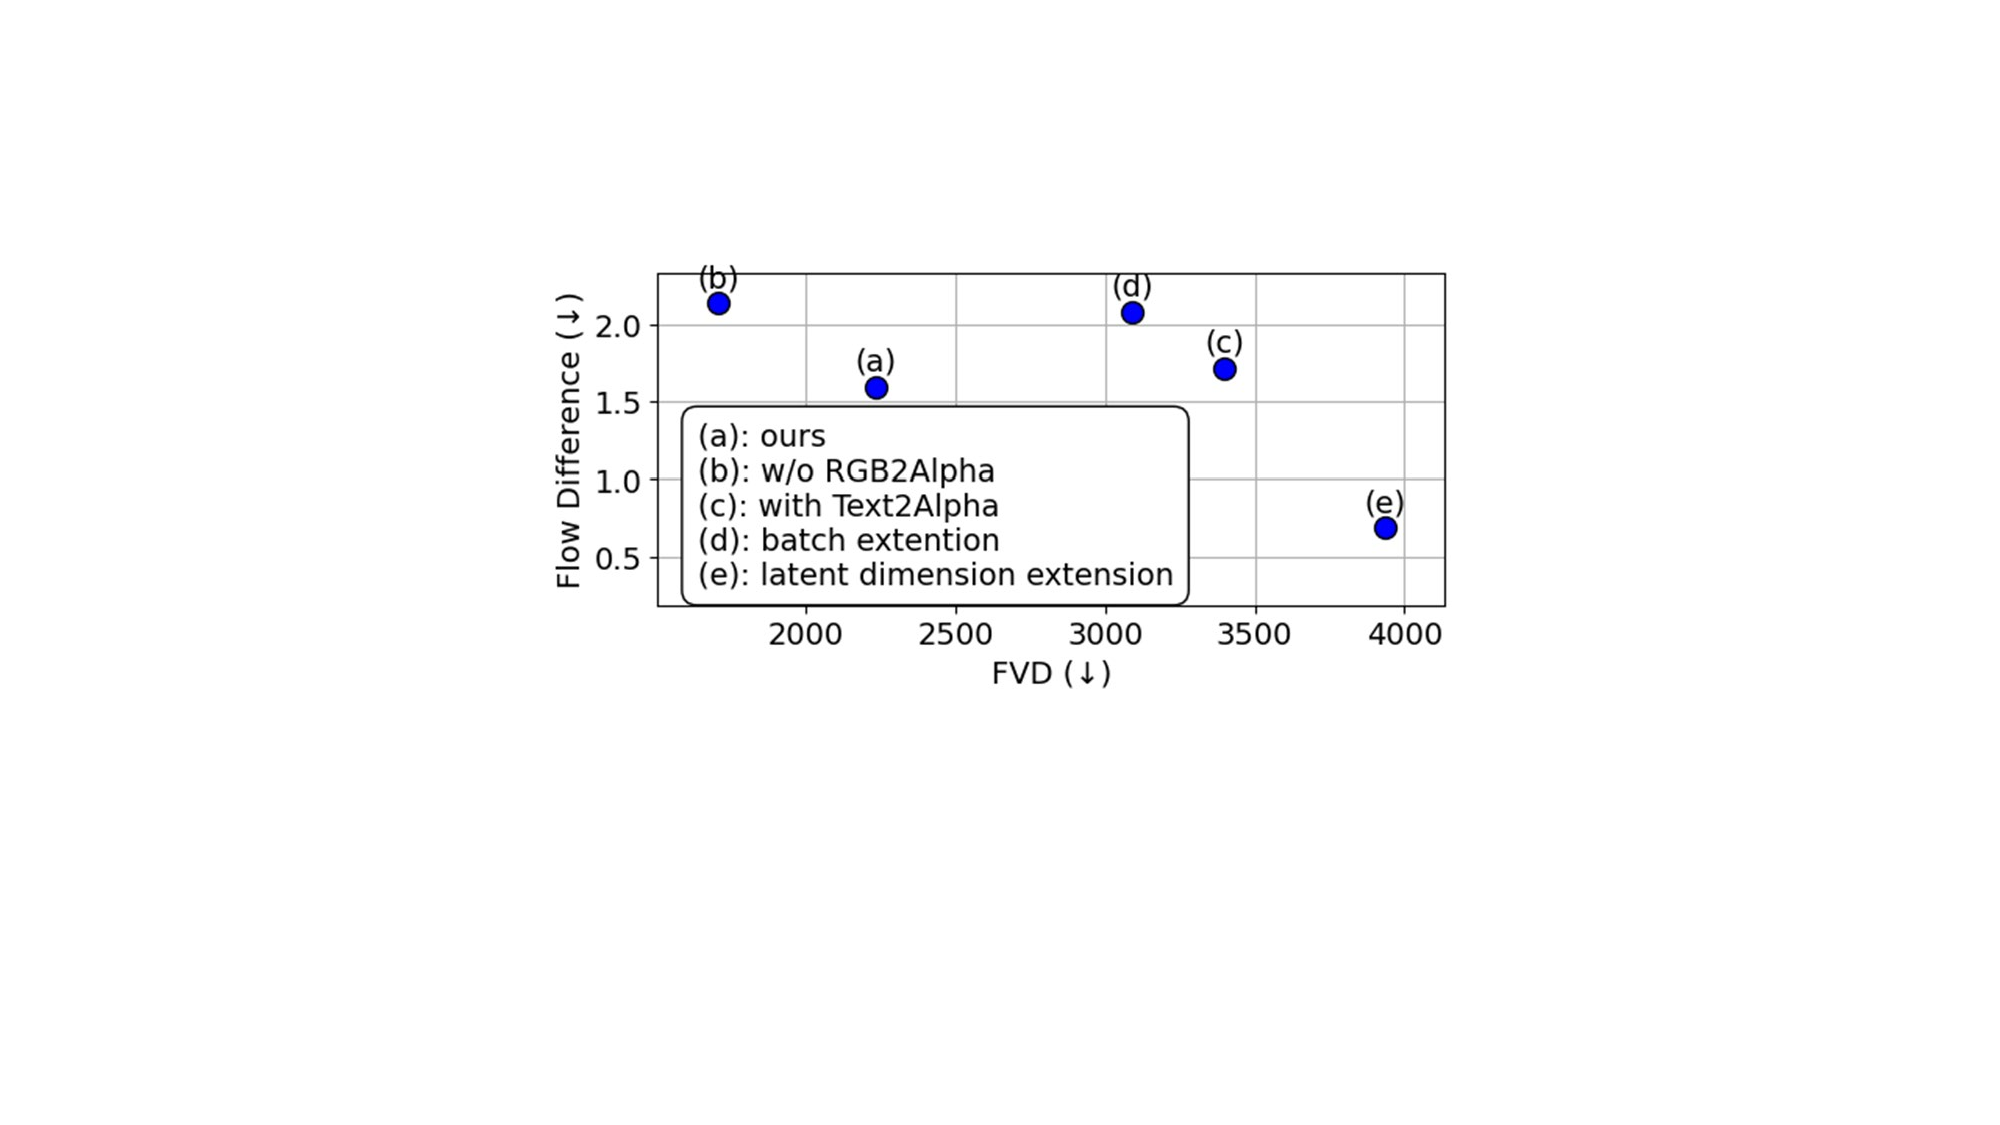
\includegraphics[width=0.9\linewidth]{figs/exp-ablation-metrics}
    \vspace{-0.1in}
    \caption{\textbf{Quantitative Evaluation}. Our approach achieves a good balance between alignment (low flow difference) and preserving generative quality (low FVD).}
    \label{fig-abaltion-metrics}
    \vspace{-0.1in}
\end{figure}
% %-------------------------------------------------------------------------
%\subsection{Limitations}
% \vspace{0.5em}
% \noindent\textbf{Limitation.} Our transformer-based method for RGBA generation incurs quadratic computational costs due to sequence expansion. However, it achieves strong results on a limited dataset. Also, numerous studies have addressed the computational overhead of long sequences, with many optimizations reducing complexity to a linear scale. To enhance the efficiency of our method, we plan to incorporate these optimizations in future work. %Additionally, our performance is shaped by the generative priors provided by the T2V model, which influence the quality and consistency of our outputs.










